\chapter{\IfLanguageName{dutch}{Over de metingen}{About the measurements}}
\label{ch:metingen}

\section{De gebruikstijd bij bepaalde opdrachten}
\label{sec:gebruikstijd}

Een van de gemeten variabelen was de gebruikstijd bij bepaalde opdrachten. Er werd gemeten hoe lang de participant erover deed om bepaalde opdrachten te voltooien. De opdrachten waren bij alle participanten gelijk:
\begin{enumerate}
    \item Enkele instellingen wijzigen
    \item Een nieuw spaardoel toevoegen
    \item Een bedrag toevoegen aan een spaardoel
    \item Een reeds voltooid spaardoel verwijderen
    \item Een berekening met de ingebouwde calculator
    \item Een groot bedrag toevoegen aan een spaardoel\\\textit{Deze opdracht werd pas na een korte onderbreking uitgevoerd.}
\end{enumerate}

In tabellen~\ref{tab:beschrijving-tijden-zonder-elementen} en \ref{tab:beschrijving-tijden-met-elementen} worden de gemiddelden en standaardafwijkingen van de gemeten tijden weergegeven. Hier kan men waarnemen dat er eventueel een verschil zal zijn in tijden tussen de groep die de opdrachten zonder onboarding en help-elementen voltooiden en de groep die de opdrachten met voltooiden. Het verschil wordt in hoofdstuk~X bewezen. % TODO

\begin{table}[h]
    \centering
    \begin{tabular}{rcc}
        \multicolumn{1}{l}{} & \multicolumn{2}{c}{\textit{Tijd in seconden}} \\
        \multicolumn{1}{r|}{\textbf{Opdracht}} & \textbf{Gemiddelde} & \textbf{Standaardafwijking} \\ \hline
        \multicolumn{1}{r|}{Instellingen} & 24.08 & 12.87 \\
        \multicolumn{1}{r|}{Spaardoel toevoegen} & 48.83 & 20.7 \\
        \multicolumn{1}{r|}{Bedrag toevoegen} & 35.67 & 18.52 \\
        \multicolumn{1}{r|}{Spaardoel verwijderen} & 65.25 & 57.46 \\
        \multicolumn{1}{r|}{Berekening} & 40.33 & 17.5 \\
        \multicolumn{1}{r|}{Groot bedrag toevoegen} & 47.25 & 35.76
    \end{tabular}
    \caption{Beschrijving van tijden zonder het gebruik van onboarding en help-elementen}
    \label{tab:beschrijving-tijden-zonder-elementen}
\end{table}

\begin{table}[h]
    \centering
    \begin{tabular}{rcc}
        \multicolumn{1}{l}{} & \multicolumn{2}{c}{\textit{Tijd in seconden}} \\
        \multicolumn{1}{r|}{\textbf{Opdracht}} & \textbf{Gemiddelde} & \textbf{Standaardafwijking} \\ \hline
        \multicolumn{1}{r|}{Instellingen} & 15.31 & 7.39 \\
        \multicolumn{1}{r|}{Spaardoel toevoegen} & 34.92 & 13.77 \\
        \multicolumn{1}{r|}{Bedrag toevoegen} & 22.62 & 8.03 \\
        \multicolumn{1}{r|}{Spaardoel verwijderen} & 16.38 & 11.94 \\
        \multicolumn{1}{r|}{Berekening} & 26.15 & 9.33 \\
        \multicolumn{1}{r|}{Groot bedrag toevoegen} & 24.77 & 27.88
    \end{tabular}
    \caption{Beschrijving van tijden met het gebruik van onboarding en help-elementen}
    \label{tab:beschrijving-tijden-met-elementen}
\end{table}

\section{Het vragen om hulp}
\label{sec:vragen-hulp}

Niet elke participant kon elke opdracht succesvol voltooien. In figuur~\ref{fig:beschrijving-hulp} wordt procentueel weergegeven indien men hulp nodig had bij het voltooien van de opdrachten. Er wordt een onderverdeling gemaakt indien men al dan niet gebruik kon maken van onboarding en help-elementen.

\begin{figure}[h]
    \centering
    \subfloat[Instellingen]{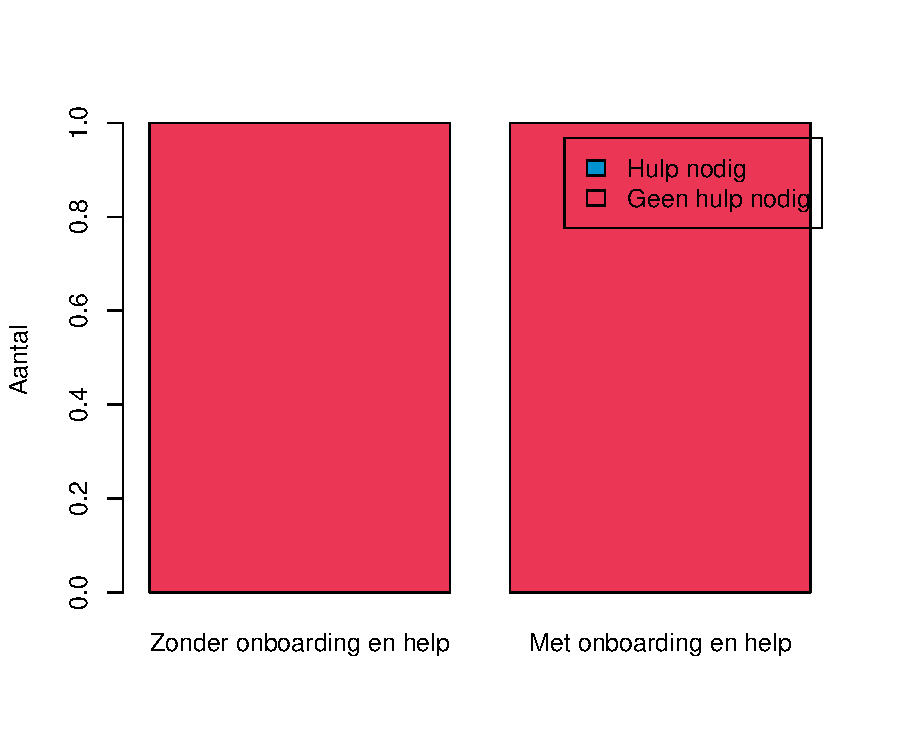
\includegraphics[width=.46\columnwidth]{beschrijving-hulp-instellingen}}
    \qquad
    \subfloat[Spaardoel toevoegen]{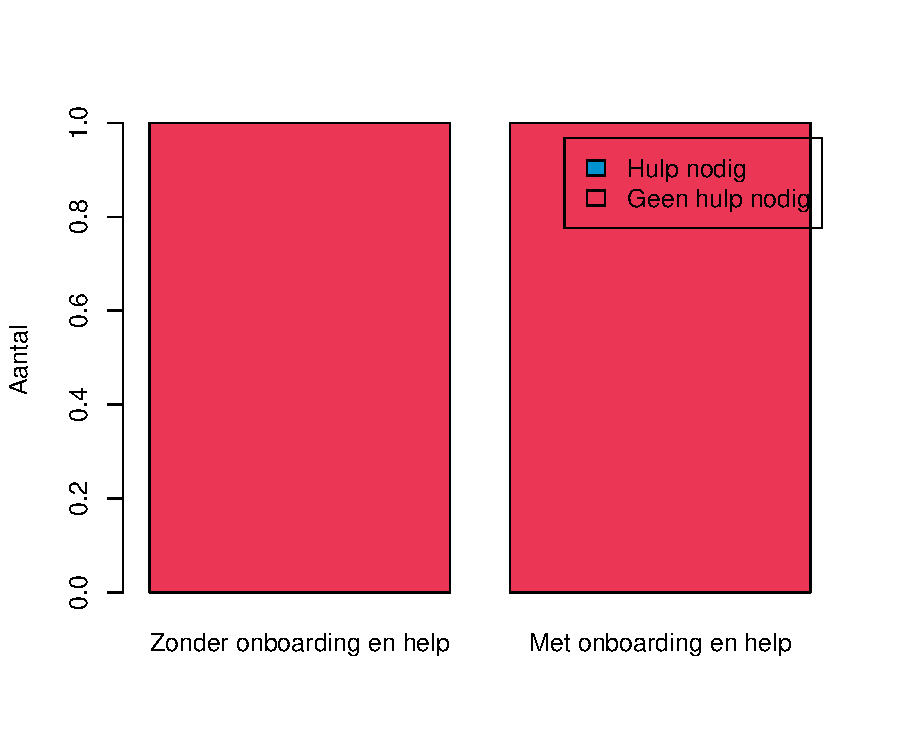
\includegraphics[width=.46\columnwidth]{beschrijving-hulp-spaardoel-toevoegen}}
    \qquad
    \subfloat[Bedrag toevoegen]{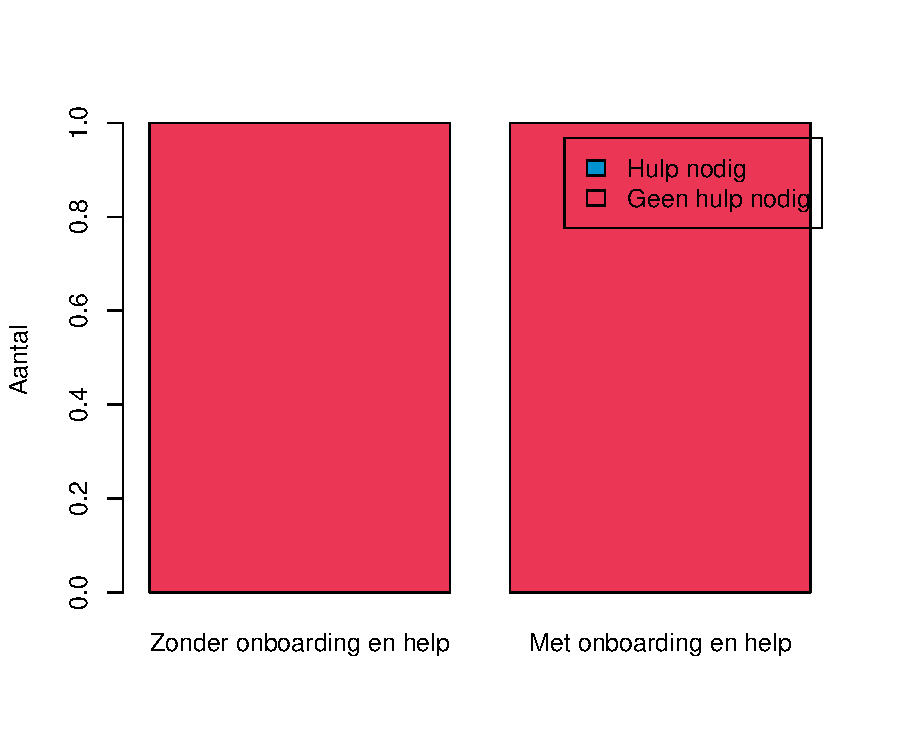
\includegraphics[width=.46\columnwidth]{beschrijving-hulp-bedrag-toevoegen}}
    \qquad
    \subfloat[Spaardoel verwijderen]{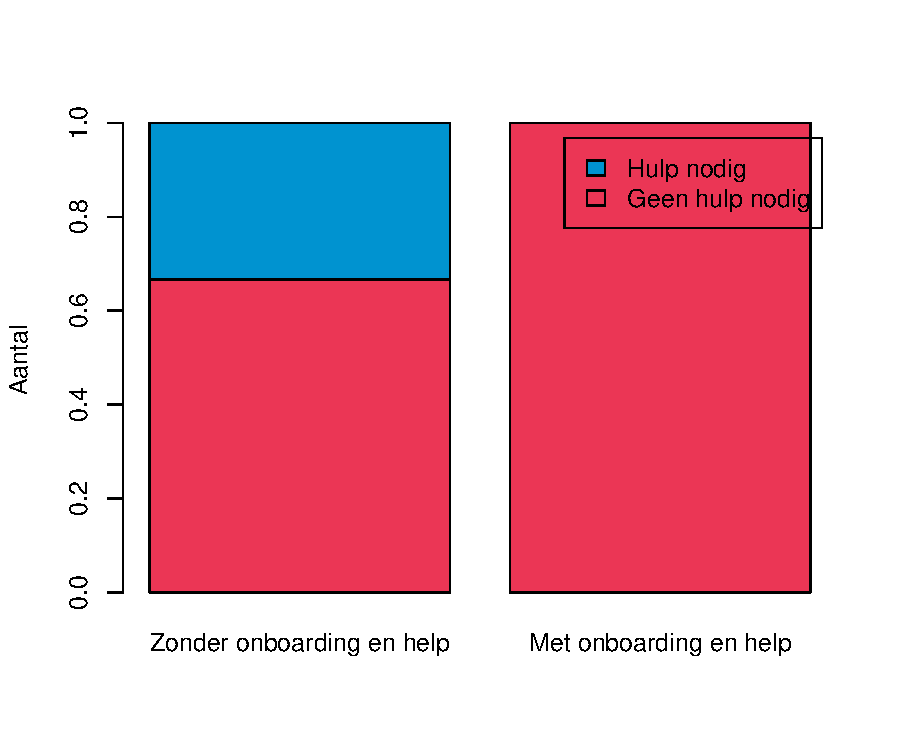
\includegraphics[width=.46\columnwidth]{beschrijving-hulp-spaardoel-verwijderen}}
    \qquad
    \subfloat[Berekening]{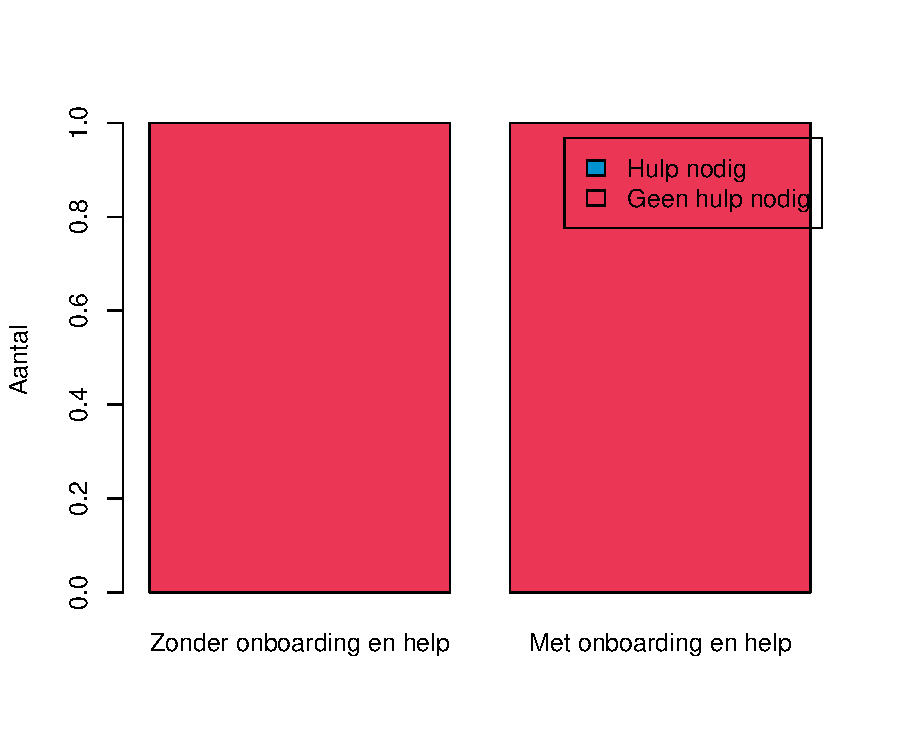
\includegraphics[width=.46\columnwidth]{beschrijving-hulp-berekening}}
    \qquad
    \subfloat[Groot bedrag toevoegen]{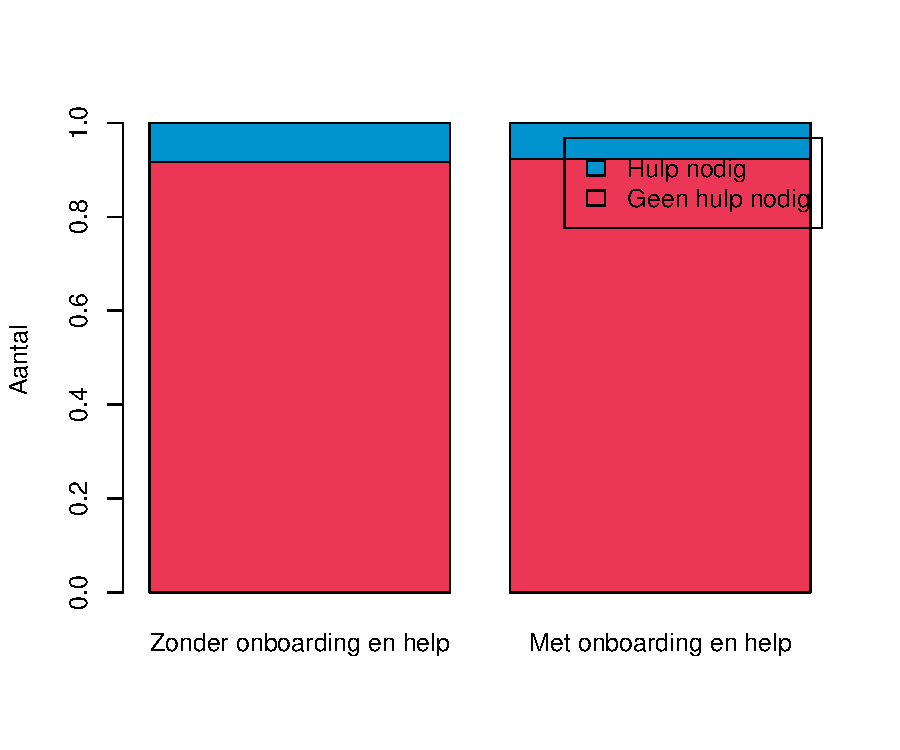
\includegraphics[width=.46\columnwidth]{beschrijving-hulp-groot-bedrag-toevoegen}}
    \caption{Indien de participant hulp nodig had bij het voltooien van de opdrachten}
    \label{fig:beschrijving-hulp}
\end{figure}

Uit figuur~\ref{fig:beschrijving-hulp} kan men afleiden dat er slechts voor sommige opdrachten hulp gevraagd werd.

\section{Gebruik van de voorziene functionaliteiten}
\label{sec:gebruik-functionaliteiten}

Men kan op verschillende manieren een bedrag toevoegen aan een spaardoel (zie figuur~\ref{fig:piggy:add-amount}). De snelste manier is door een slider te verschuiven tot het bedrag correct is en dan op de grote knop ``Add money'' te drukken. Deze slider gaat slechts tot een maximum van 50. Wanneer de gebruiker een hoger bedrag wil toevoegen moet deze op de knop met het ``+''-symbool drukken. Dit werd uitgelegd in de rondleiding doorheen de applicatie.

\begin{figure}[h!]
    \centering
    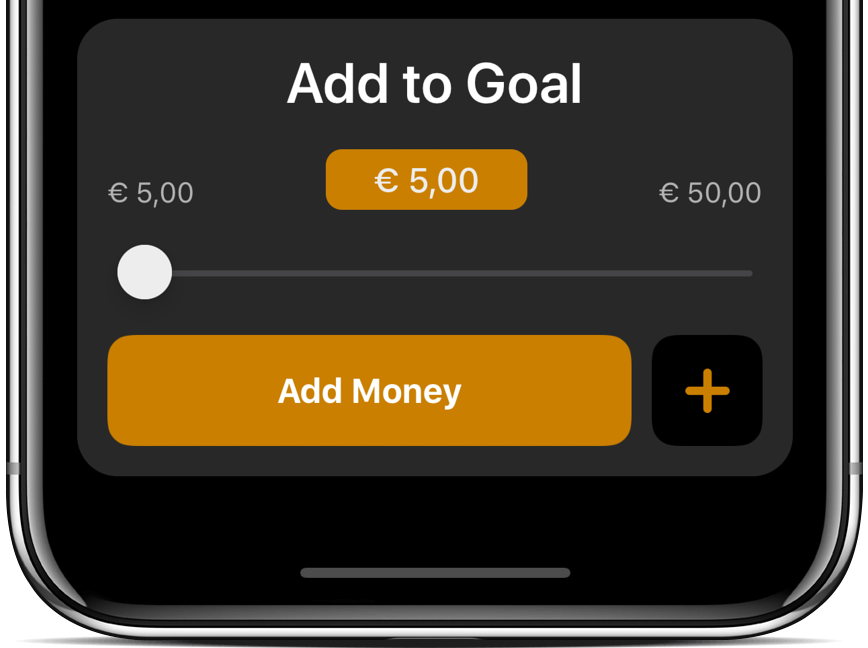
\includegraphics[width=.5\columnwidth]{piggy-add-amount}
    \caption{Verschillende manieren om een bedrag aan een spaardoel toe te voegen}
    \label{fig:piggy:add-amount}
\end{figure}

In figuur~\ref{fig:beschrijving-plus} wordt procentueel weergegeven hoeveel participanten gebruik hebben gemaakt van het ``+''-symbool bij de opdrachten die vereisten om een bedrag toe te voegen.

\begin{figure}[h]
    \centering
    \subfloat[Bedrag toevoegen]{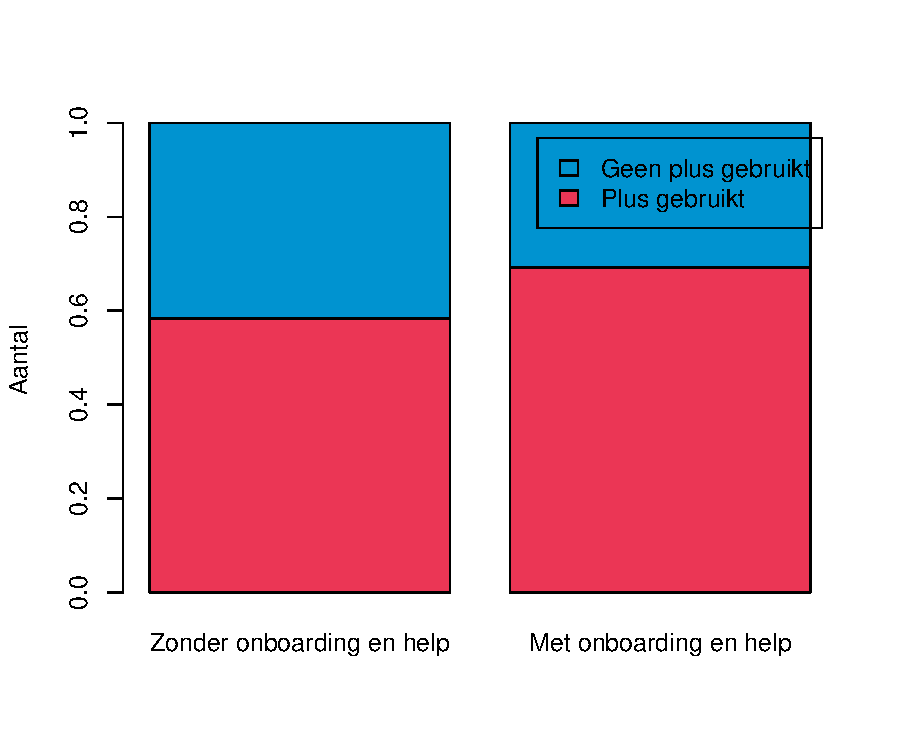
\includegraphics[width=.46\columnwidth]{beschrijving-plus-bedrag-toevoegen}}
    \qquad
    \subfloat[Groot bedrag toevoegen]{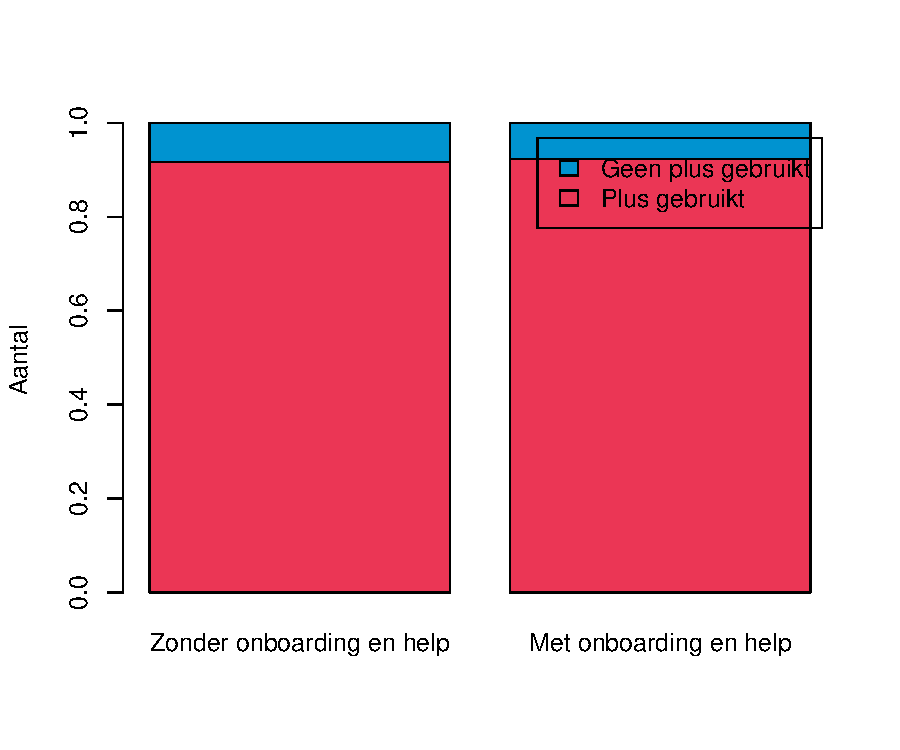
\includegraphics[width=.46\columnwidth]{beschrijving-plus-groot-bedrag-toevoegen}}
    \caption{Indien de participant hulp nodig had bij het voltooien van de opdrachten}
    \label{fig:beschrijving-plus}
\end{figure}

\section{De SUS-score}
\label{sec:sus}

\section{Voorkeur voor onboarding en help-elementen}
\label{sec:voorkeur-onboarding}

De participanten werden na afloop gevraagd indien ze de proof-of-concept applicatie liefst gebruikten indien de onboarding en help-elementen aanwezig waren. De resultaten van deze vraag worden procentueel weergegeven in figuur~\ref{fig:beschrijving-finds-better}.

\begin{figure}[h]
    \centering
    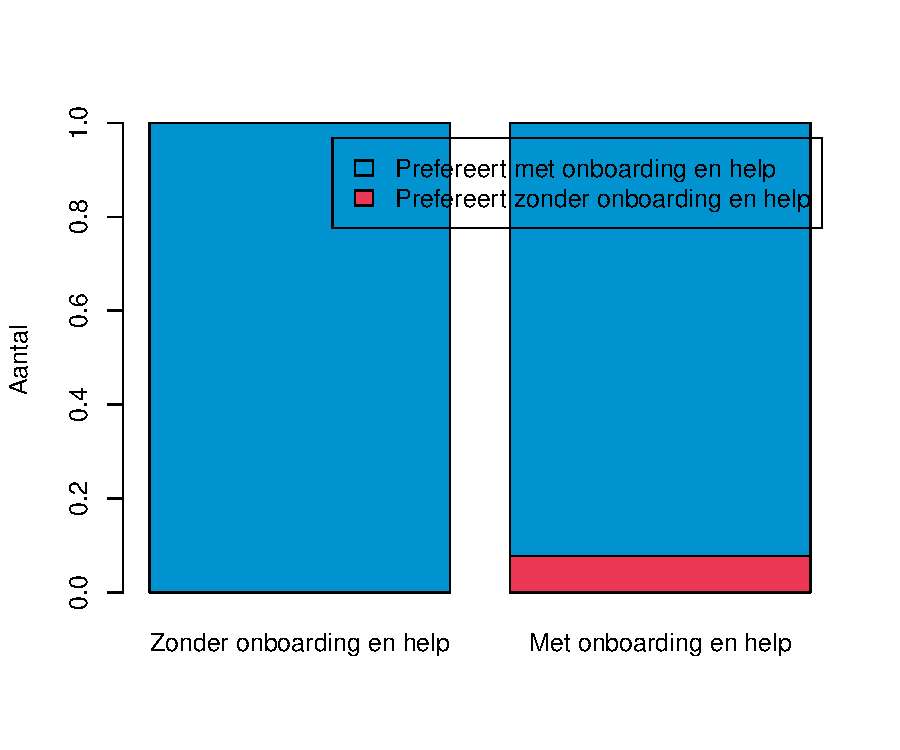
\includegraphics[width=.46\columnwidth]{beschrijving-finds-better}
    \caption{De voorkeur van de participant: een applicatie met of zonder onboarding en help-elementen}
    \label{fig:beschrijving-finds-better}
\end{figure}

Participanten die de applicatie prefereren zonder de onboarding en help-elementen maken deze keuze omdat de applicatie voor hun eenvoudig en duidelijk genoeg was. Indien de applicatie enkele meer ingewikkelde functionaliteiten zou hebben, zouden ook zij liever geholpen worden doorheen de applicatie.

\section{Voorkeur voor help-sectie}
\label{sec:voorkeur-help}

Er werd de participanten een voorbeeld getoond van de help-sectie in de applicatie (zie figuur~\ref{fig:piggy:help}). Hierover werd aan de participant gevraagd indien deze gebruik zou maken van een gelijkaardige help-sectie in deze of andere applicaties. De resultaten van deze vraag worden procentueel weergegeven in figuur~\ref{fig:beschrijving-would-use-help}.

\begin{figure}[h]
    \centering
    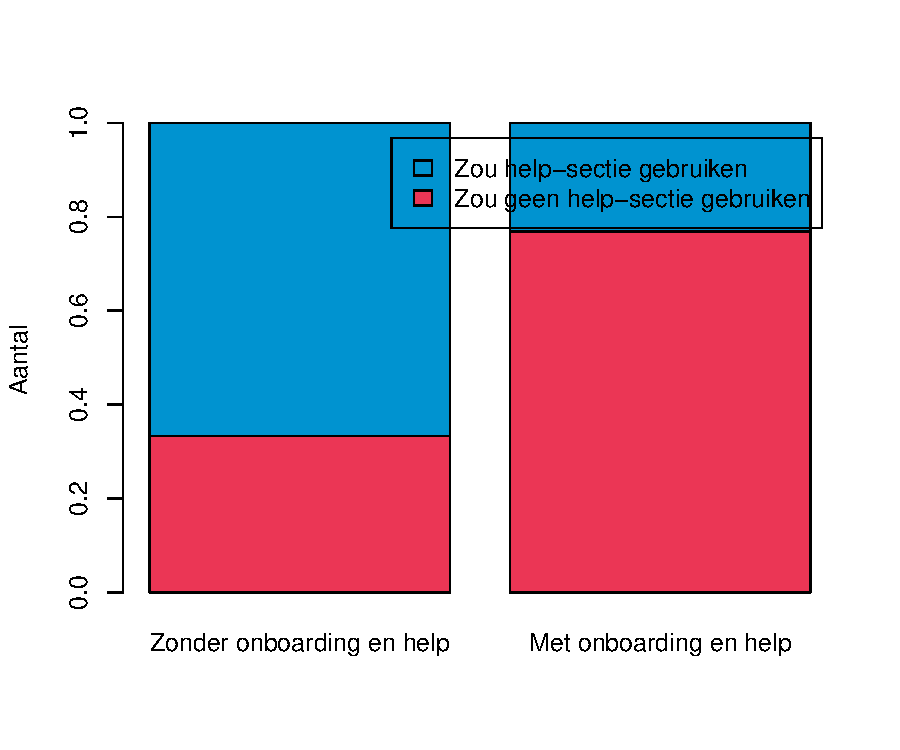
\includegraphics[width=.46\columnwidth]{beschrijving-would-use-help}
    \caption{Indien de participant zichzelf de help-sectie ziet gebruiken}
    \label{fig:beschrijving-would-use-help}
\end{figure}

\section{De gebruiksduur en/of levensduur van de applicatie}
\label{sec:gebruiksduur}

